\section{Erkenntnisse bei der Variation von \texorpdfstring{$k_{max}$}{kmax}}

Es wird davon ausgegangen, dass sich mit der Variation von $k_{max}$ bei der 
Welle keine grossen Ver"anderungen einstellen. Die Werte werden immer ab einem 
gewissen Punkt ins Positive oder Negative explodieren, da das $x^k$ irgendwann 
dominiert. Mit $k_{max}$ wird die Anzahl der Summanden bezeichnet, die f"ur die 
Berechnung der Potenzreihe verwendet werden. 

\begin{equation*}
y(x) = a_0 + a_1x 
-\sum_{k=2}^{k_{max}}\frac{1}{k(k-1)}(aa_{k-4}+ba_{k-3}+ca_{k-2})x^k
\end{equation*}

Es werden die Startbedingungen gem"ass den Gleichungen 
\ref{wellen:Startbedingungen1} festgelegt.

\begin{equation}
	\begin{split}
		a_0 &= 1\\
		a_1 &= 0\\
		a &= 1\\
		b &= 0\\
		c &= -1
	\end{split}
	\label{wellen:Startbedingungen1}
\end{equation}

Auf folgenden Grafiken wird veranschaulicht, was mit der Welle passiert, wenn 
das $k_{max}$ jeweils um 30 vergr"ossert wird. Es wird dann "uberpr"uft, ob 
sich die Behauptung der kleinen Ver"anderungen als wahr herausstellt.

\begin{center}
	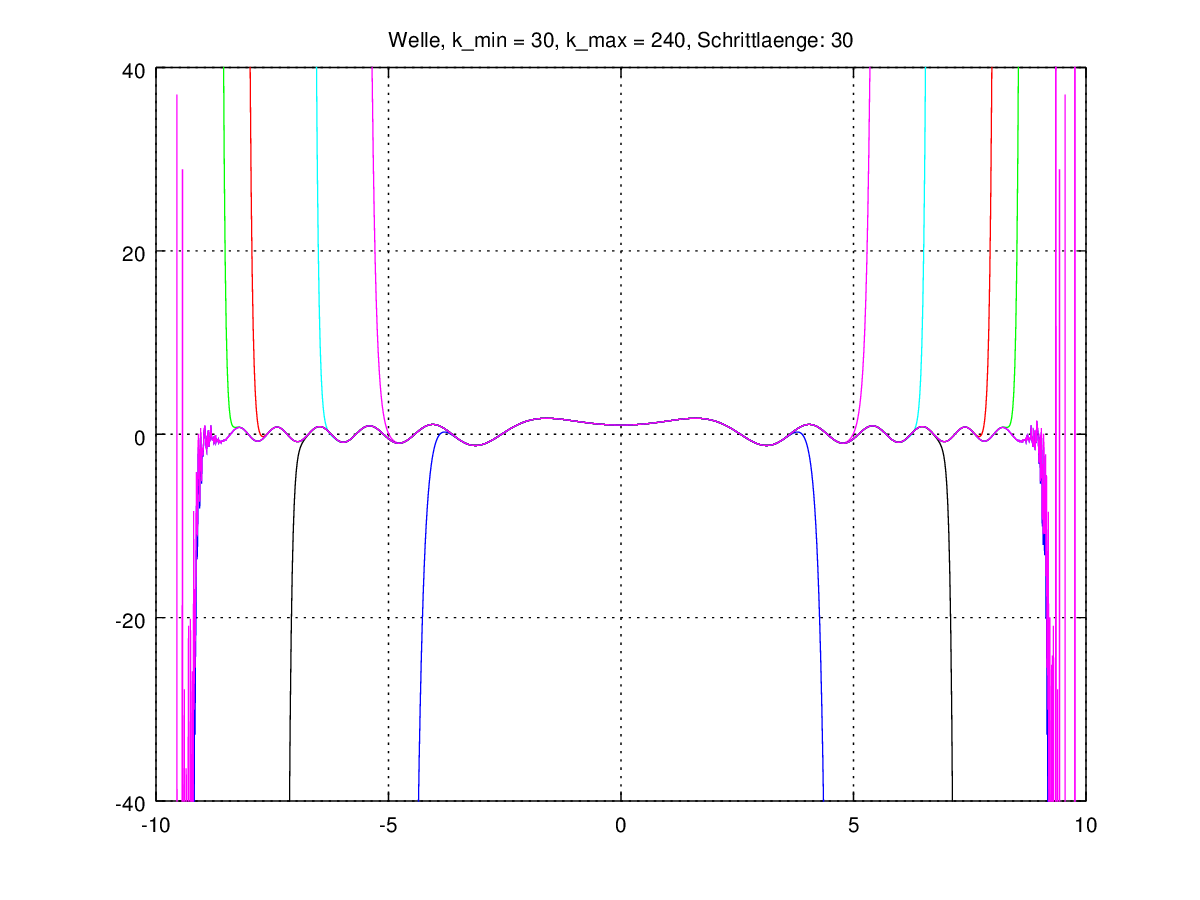
\includegraphics[scale=0.69]{./wellen/images/kmax/krangewaveeven.png}
\end{center}

Die Behauptung, dass der Wert irgendwann explodiert, ist, wie ersichtlich, 
wahr. Der Punkt wo die Werte gegen $\infty$ gehen verschiebt sich immer mehr 
nach rechts, zu gr"osseren $x$-Werten. Dies wird dadurch erkl"art, dass es 
immer l"anger geht, bis der $x^k$-Term dominiert. Je mehr der $k_{max}$-Wert 
gesteigert wird, umso besser wird die Approximation an die Welle. Ab einer 
gewissen Gr"osse von $k_{max}$ kann das Programm die Werte nicht mehr genau 
bestimmen, was die unregelm"assigen Ausschl"age erkl"art.

Aufgrund dieser Messungen wird $x$ f"ur die weiteren Berechnungen auf $x \in 
[-8;8]$ und $k_{max}$ auf 180 beschr"ankt, damit die $y$-Werte nicht 
explodieren und keine unkontrollierten Messwerte entstehen.

Mit den in diesem Kapitel festgelegten Startbedingungen und Einschr"ankungen 
ergibt dies folgende Grafik:
\begin{center}
	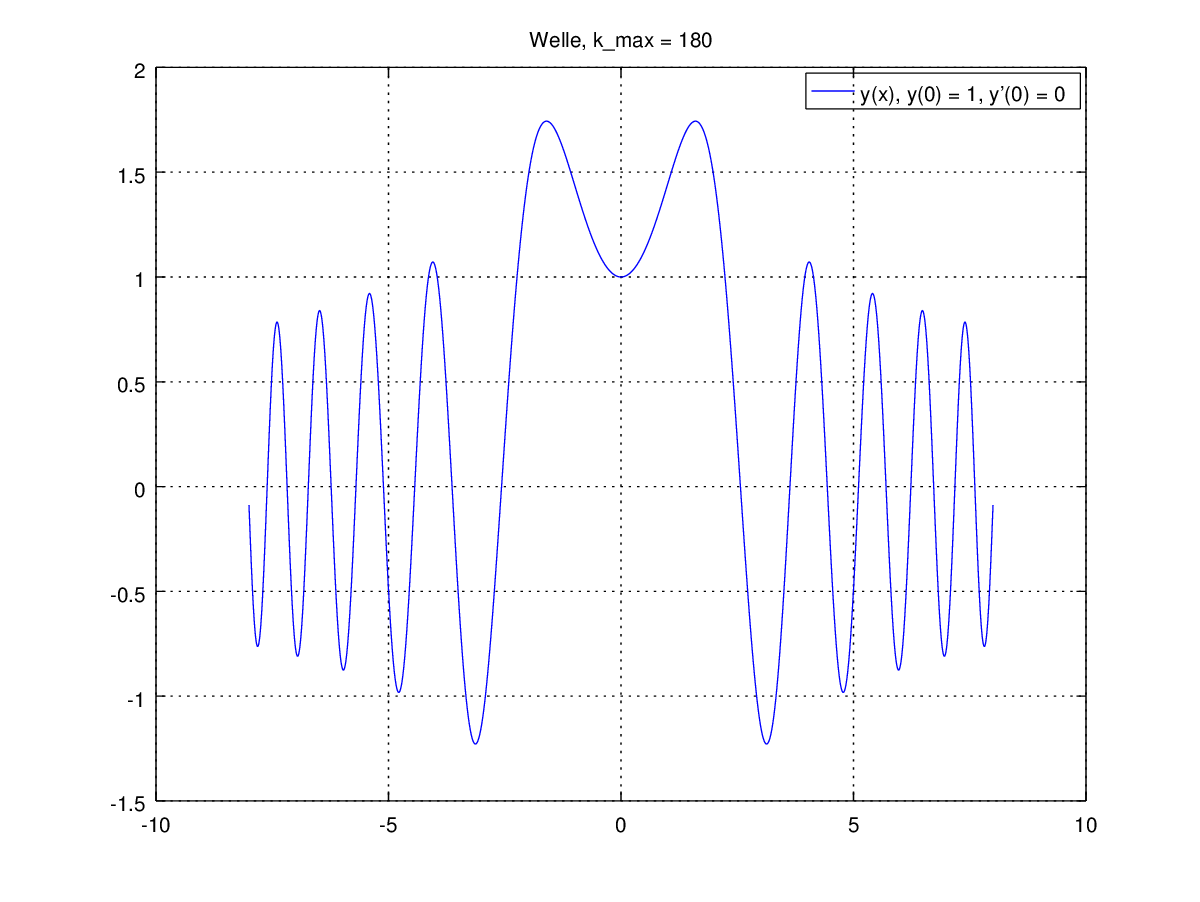
\includegraphics[scale=0.69]{./wellen/images/kmax/ak180-88wave.png}
\end{center}

\section{Erkenntnisse bei der Variation von \texorpdfstring{$a$}{a}, 
\texorpdfstring{$b$}{b} und \texorpdfstring{$c$}{c}}

Die Anfangsbedingungen $a_0$ und $a_1$ k"onnen beliebig festgelegt werden. Da 
sich die Wellen im betrachteten Fall um den Entwicklungspunkt $x_0=0$ bewegen, 
beschreibt das $a_0$ den y-Achsenabschnitt und das $a_1$ die Steigung im Punkt 
$y(0)$. Die gew"ahlten Werte von $a_0$ und $a_1$ sind jeweils in der Grafik 
ersichtlich.

\subsection{Eliminierung von $a$ und $b$}
\label{wellen:Eliminierungab}

Zu Beginn wird das vorgegebene, parabelf"ormige Geschwindigkeitsprofil 
n"aherungsweise in eine Konstante umgewandelt indem $a$ verschwindend klein 
gew"ahlt wird und $b$ gleich $0$ gesetzt wird. Die beiden Variablen werden also 
eliminiert und folgende Differentialgleichung wird betrachtet:

\begin{equation}
	y''+ cy = 0.
	\label{wellen:lineareDGL}
\end{equation}


F"ur positive Werte von c kann die L"osung dieser Gleichung 
\ref{wellen:lineareDGL} mit dem charakteristischen Polynom bestimmt werden. 
Die L"osungen des charakteristischen Polynoms

\begin{equation}
	p(\lambda) = [(\lambda+\mu)^2+\omega^2] =0
	\label{wellen:charakteristischesPolynom}
\end{equation}

sind

\begin{equation}
	\begin{split}
	y_1 &= C_1e^{-\mu x}\cos(\omega x) \\
	y_1 &= C_2e^{-\mu x}\sin(\omega x).
	\end{split}
	\label{wellen:lsgcharakteristischesPolynom}
\end{equation}

Das zur Gleichung \ref{wellen:lineareDGL} geh"orende charakteristische Polynom 
ist gem"ass \ref{wellen:charakteristischesPolynom}

\begin{equation*}
	p(\lambda) = [\lambda^2 + c] =0.
\end{equation*}

Somit folgt die allgemeine L"osung der Differentialgleichung 
\ref{wellen:lineareDGL} gem"ass \ref{wellen:lsgcharakteristischesPolynom}

\begin{equation}
	y(x) = C_1 \cos(\sqrt{c}x) + C_2 \sin(\sqrt{c}x)
	\label{wellen:LsglineareDGL}
\end{equation}

Um die Konstanten $C_1$ und $C_2$ zu bestimmen m"ussen die Anfangsbedingungen 
$a_0$ und $a_1$ bekannt sein. Um die Abh"angigkeit aufzuzeigen, muss zuerst die 
erste Ableitung der L"osung \ref{wellen:LsglineareDGL} aufgestellt werden.

\begin{equation}
	y'(x)=-C_1 \sqrt{c} \sin(\sqrt{c}x) + C_2 \sqrt{c} \cos(\sqrt{c}x)
\end{equation}

Der Wert bei $y(0)$ ist definiert als $a_0$ und die Steigung am Punkt $y'(0)$ 
ist das $a_1$. Setzt man $x=0$ in die L"osungsgleichung 
\ref{wellen:LsglineareDGL} ein, k"onnen $C_1$ und $C_2$ bestimmt werden.

\begin{equation}
	\begin{split}
		y(0) = C_1 = a_0 &\Leftrightarrow C_1 = a_0 \\
		y'(0) = C_2 \sqrt{c} = a_1 &\Leftrightarrow C_2 = \frac{a_1}{\sqrt{c}}
	\end{split}
	\label{wellen:KonstantenC1C2}
\end{equation}

Setzt man diese Konstanten \ref{wellen:KonstantenC1C2} in die L"osungsgleichung 
\ref{wellen:LsglineareDGL} 
ein, ergibt sich die Gleichung, die sich mit den Startangaben, die definiert 
werden, f"ur positive $c$-Werte berechnen l"asst.

\begin{equation}
	y(x) = a_0 \cos(\sqrt{c}x) + \frac{a_1}{\sqrt{c}} \sin(\sqrt{c}x)
	\label{wellen:LSGleichung}
\end{equation}

In den folgenden zwei Grafiken werden die zwei Grundfunktionen von ``reinem''
Sinus (erste Grafik) und Cosinus (zweite Grafik) aufgezeigt. Daf"ur muss 
entweder $a_0$ oder $a_1$ gleich Null gesetzt werden.

\noindent
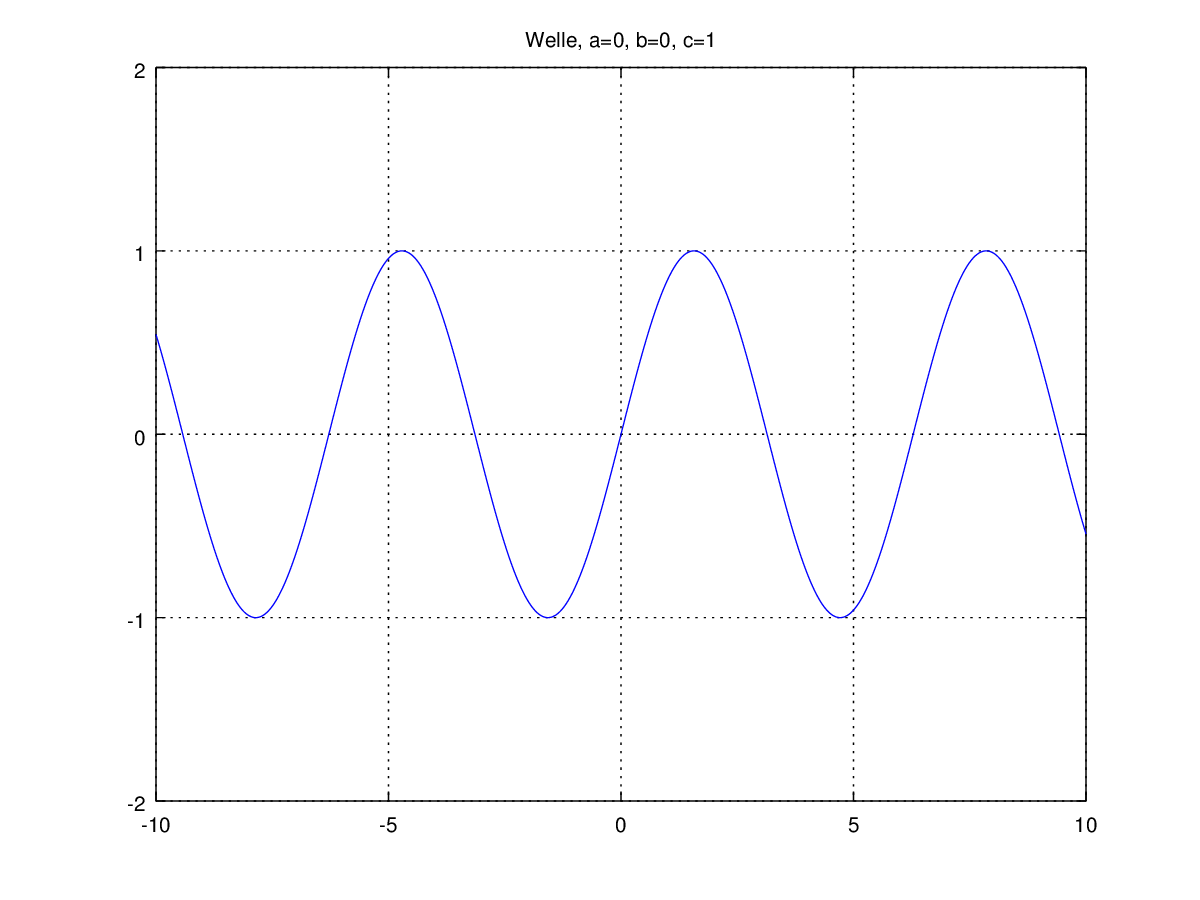
\includegraphics[scale=0.35]{./wellen/images/basicfunctions/sin.png}
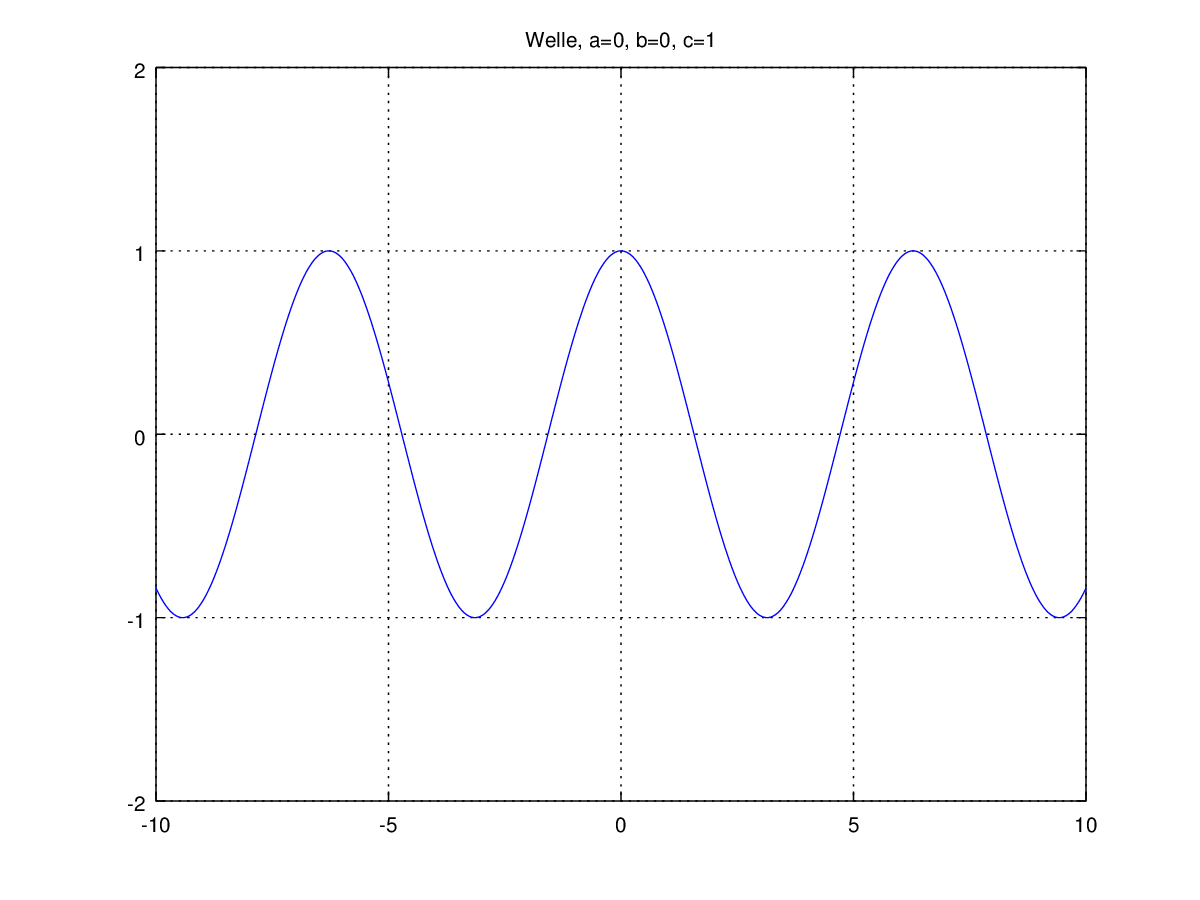
\includegraphics[scale=0.35]{./wellen/images/basicfunctions/cos.png}

F"ur negative Werte von c kann die L"osungsgleichung \ref{wellen:LSGleichung} 
zwar auch verwendet werden, es entstehen aber imagin"are Faktoren durch die 
negativen Wurzelwerten. Die imagin"are Einheit $i$ ist definiert als

\begin{equation}
	i = \sqrt{-1}.
	\label{wellen:imaginaereEinheit}
\end{equation}

Wird dieser Wurzelwert \ref{wellen:imaginaereEinheit} bei jedem negativen Wert 
von $c$ ausgeklammert, ergibt sich die L"osungsgleichung.

\begin{equation}
	\begin{split}
	y(x) &= a_0 \cos(i\sqrt{|c|}x) + \frac{a_1}{i\sqrt{|c|}}\sin(i\sqrt{|c|}x) 
	\\
	\Leftrightarrow
	y(x) &= a_0 \cos(i\sqrt{|c|}x) - i\frac{a_1}{\sqrt{|c|}}\sin(i\sqrt{|c|}x)
	\end{split}	
	\label{wellen:LSGnegcWerte}
\end{equation}

Die Definitionen vom Sinus Hyperbolicus und Cosinus Hyperbolicus lauten:

\begin{equation*}
	\begin{split}
	\sinh(x) &= \frac{1}{2} (e^x - e^{-x}) = -i \sin(ix)\\
	\cosh(x) &= \frac{1}{2} (e^x + e^{-x}) = \cos (ix)
	\end{split}
\end{equation*}

Werden die Definitionen mit der L"osungsformel verglichen, ist ersichtlich, 
dass es sich je nach Wahl von $a_0$ und $a_1$ um eine der beiden hyperbolischen 
Funktionen handelt. Die L"osungsgleichung ergibt sich also zu

\begin{equation}
	y(x) = a_0 \cosh(\sqrt{|c|}x) + \frac{a_1}{\sqrt{|c|}}\sinh(\sqrt{|c|}x)
	\label{wellen:LSGhyperbolFunktion}
\end{equation}

In den folgenden zwei Grafiken wird zuerst der ``reine'' Sinus Hyperbolicus und 
als zweites der ``reine'' Cosinus Hyperbolicus dargestellt.

\noindent
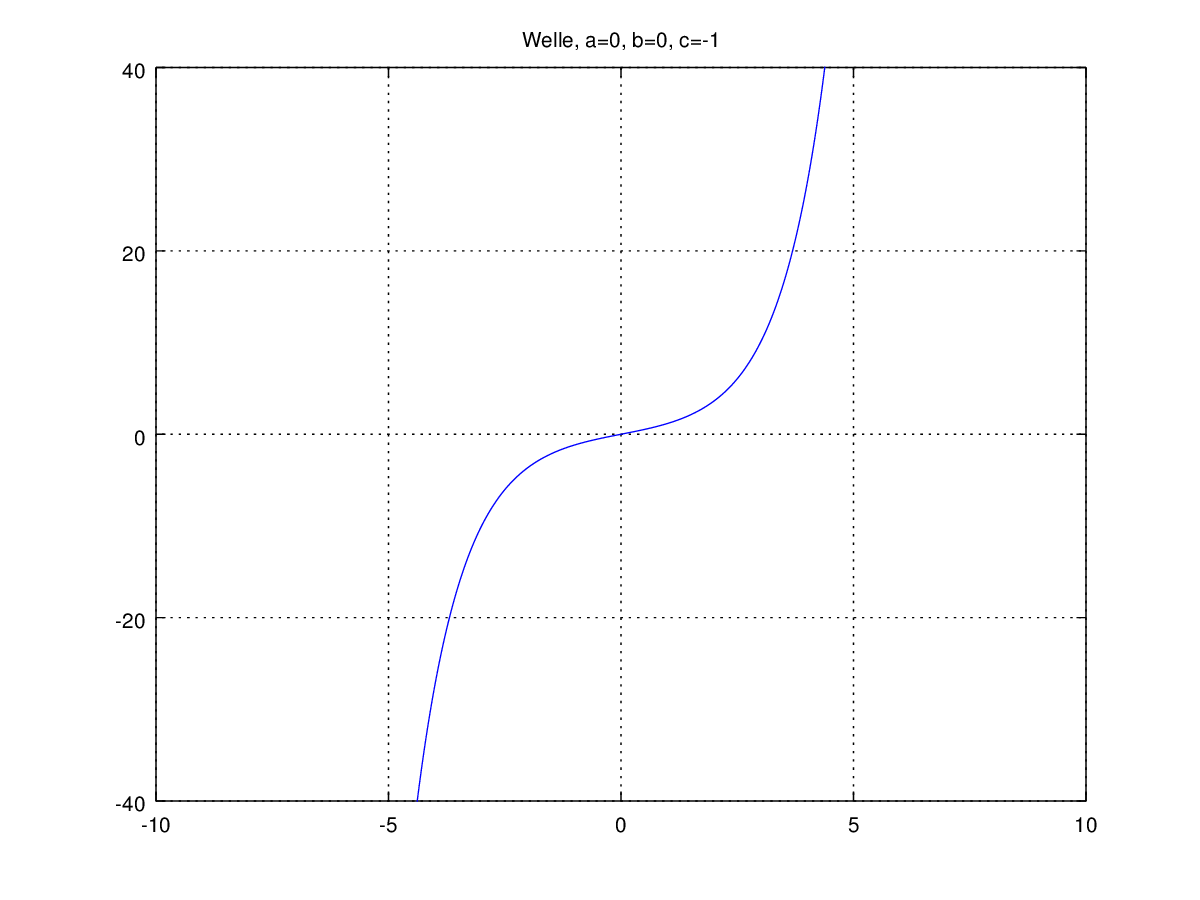
\includegraphics[scale=0.35]{./wellen/images/basicfunctions/sinh.png}
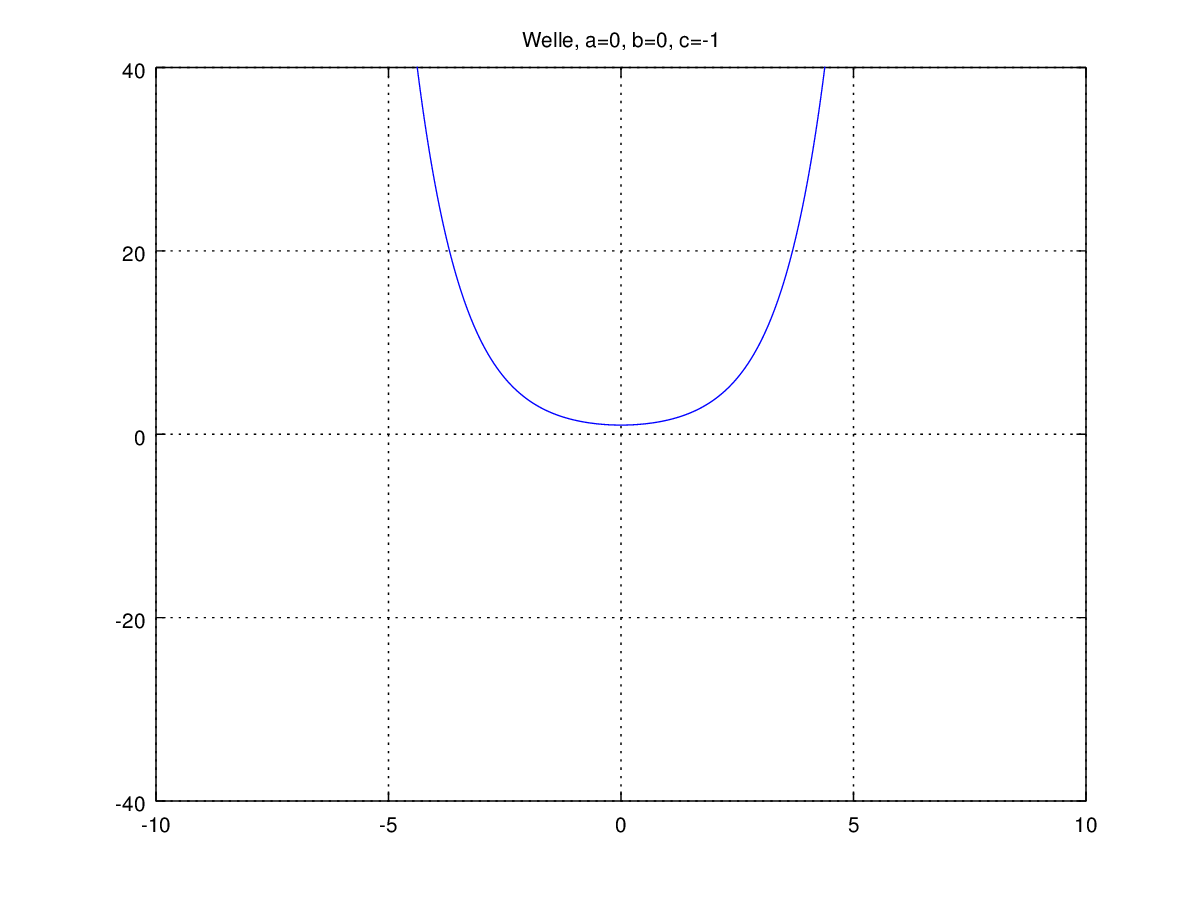
\includegraphics[scale=0.35]{./wellen/images/basicfunctions/cosh.png}

\subsection{Variation von $b$}

Als Zweites werden die Variablen $a$, $c$ und die Anfangsbedingungen 
festgehalten und nur das $b$ ver"andert. Um aufzuzeigen, was sich dabei 
ver"andert, braucht es nur die Parabelgleichung.

\begin{equation*}
	y(x) = ax^2 + bx + c
\end{equation*}

BILD VERSCH. PARABELN

Der Faktor $b$ bezweckt n"amlich, wie man in der Grafik sieht, in der Parabel 
nur eine Verschiebung in Richtung der $x$-Achse. Diese Verschiebung bedeutet in 
der betrachteten Problemstellung nur, dass sich die Schnittpunkte mit der 
$x$-Achse verschieben. Was dies bedeutet wird in einem sp"ateren Abschnitt 
erkl"art. Was aber aus der Variation mit $b$ herausgeht ist, dass wir die 
dadurch ver"anderten Eigenschaften auch mit der Variation von $c$ oder von 
$a_0$ aufzeigen k"onnen. Aus diesem Grund wird die Variabel $b$ in Fortsetzung 
immer gleich 0 gesetzt und damit vernachl"assigt. 

Die neue zu betrachtende Differentialgleichung ergibt sich damit zu:

\begin{equation} 
	y'' + (ax^2 +c)y = 0
	\label{wellen:DGLzubetrachten}
\end{equation}

\subsection{Variation von $c$}
\label{wellen:Variationc}

Als N"achstes wird untersucht, welche Auswirkungen die Variation vom 
Koeffizienten $c$ hat, wenn $a$ vorhanden ist und nicht gegen 0 geht aber 
trotzdem festgehalten wird. $a$ wird in der folgenden Betrachtung gleich 1 
gesetzt.

Der Koeffizient $c$ beschreibt den Schnittpunkt der Parabel mit der $y$-Achse 
und somit die Verschiebung in $y$-Richtung. Diese Verschiebung kann nicht, wie 
die Verschiebung in Richtung der $x$-Achse mit dem Koeffizienten $b$, 
vernachl"assigt werden. Grund daf"ur ist, dass die Wellenform vom Schnittpunkt 
der Parabel mit der $x$-Achse abh"angt. 

\noindent
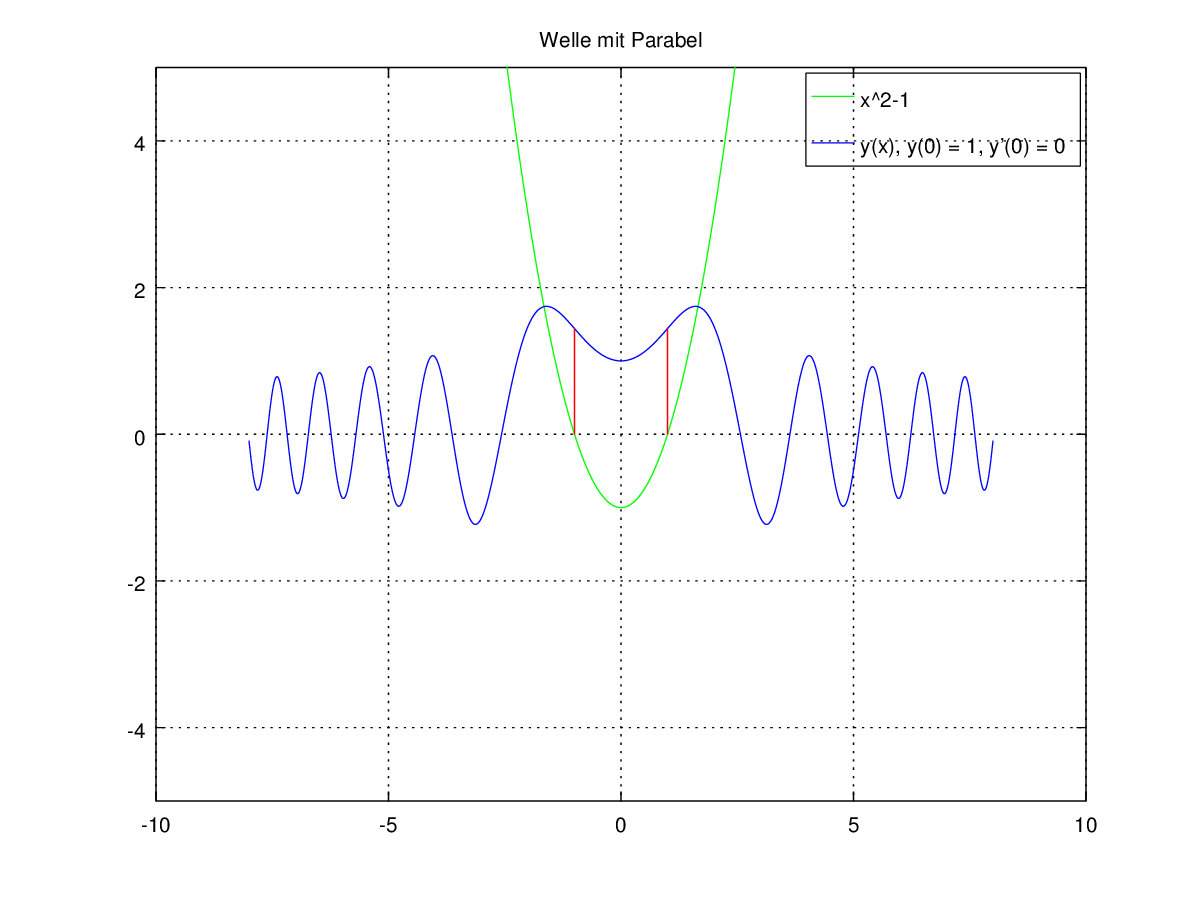
\includegraphics[scale=0.35]{./wellen/images/varc/cneg1.png}
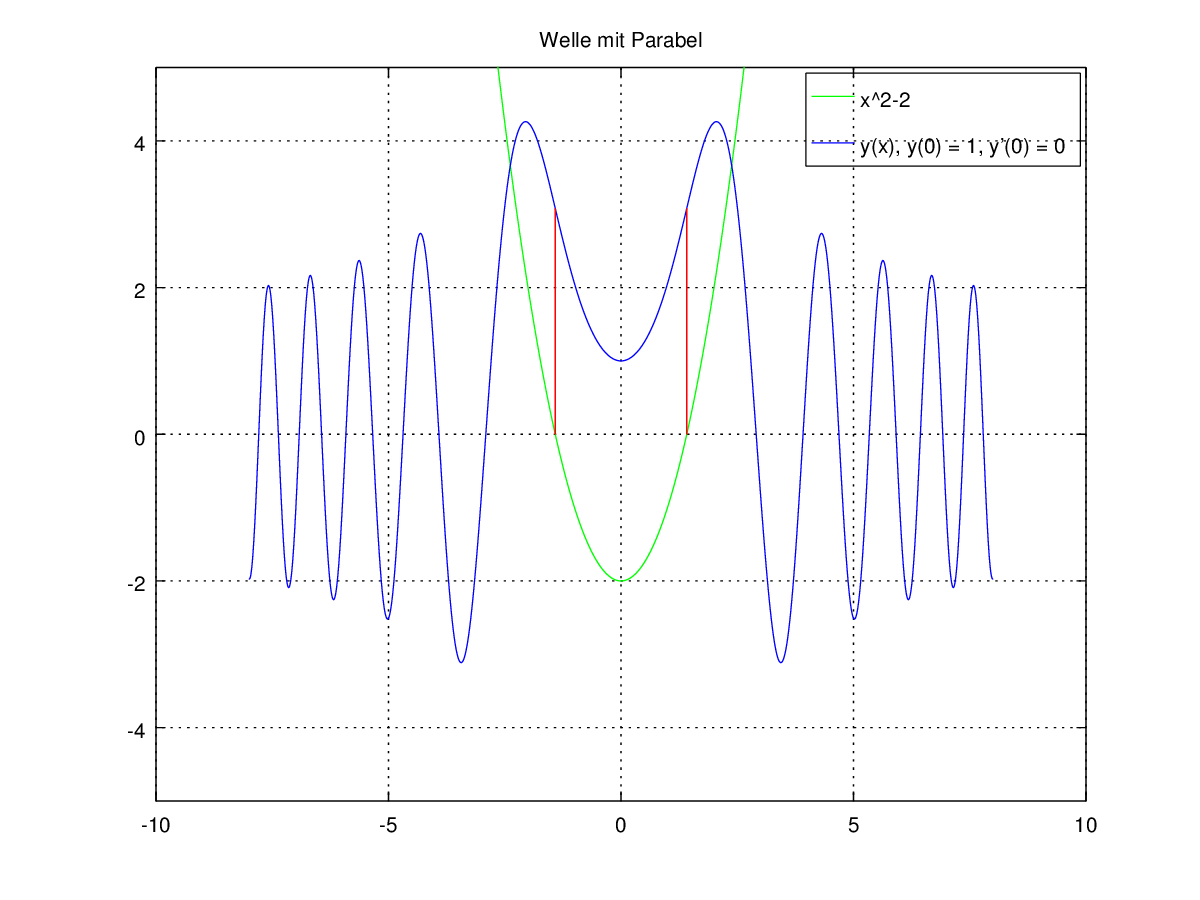
\includegraphics[scale=0.35]{./wellen/images/varc/cneg2.png}

In den zwei Grafiken werden die 
Parabeln mit zwei unterschiedlichen $y$-Achsenabst"anden und deren aus der 
Differentialgleichung \ref{wellen:DGLzubetrachten} entstehende Welle gezeigt. 
Es wird deutlich, dass es nicht die gleiche Welle gibt und dass sich beim 
Schnittpunkt der Parabel mit der $x$-Achse eine "Anderung einstellt. Dieses 
Ph"anomen wird im n"achsten Kapitel \ref{wellen:DiskussionWellenform} erkl"art. 

\subsection{Variation von $a$}
\label{wellen:Variationa}

Zum Schluss wird der Koeffizient $a$ variiert, was zur Folge hat, dass die 
Parabel schl"anker oder enger wird. Dadurch verschiebt sich auch der 
Schnittpunkt der Parabel mit der $x$-Achse und somit auch der Umschlagspunkt, 
der im Kapitel \ref{wellen:Variationc} schon ersichtlich war. 

...